
%{{第四十八回}}{第四十八回}}

\chapter{滥情人情误思游艺\hspace{.5em}慕雅女雅集苦吟诗}
{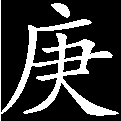
\includegraphics[width=3mm]{../Images/00004}题曰``柳湘莲走他乡'',必谓写湘莲如何走,今却不写,反细写阿呆兄之游艺,了却柳湘莲之分内走者而不细写其走,反写阿呆不应走而写其走,文牵歧路,令人不识者如此。}

{至``情小妹''回中,方写湘莲文字,真神化之笔。}

{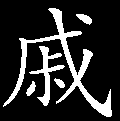
\includegraphics[width=3mm]{../Images/00005}心地聪明性自灵,喜同雅品讲诗经,姣柔倍觉可怜形。 皓齿朱唇真袅袅,痴情专意更娉娉,宜人解语小星星。}

且说薛蟠听见如此说了,气方渐平。三五日后,疼痛虽愈,伤痕未平,只装病在家,愧见亲友。

展眼已到十月,因有各铺面伙计内有算年账要回家的,少不得家内治酒饯行。内有一个张德辉,年过六十,自幼在薛家当铺内揽总,家内也有二三千金的过活,今岁也要回家,明春方来。因说起``今年纸札香料短少,明年必是贵的。明年先打发大小儿上来当铺内照管,赶端阳前我顺路贩些纸札香扇来卖。除去关税花销,亦可以剩得几倍利息。''薛蟠听了,心中忖度:``我如今捱了打,正难见人,想着要躲个一年半载,又没处去躲。天天装病,也不是事。况且我长了这么大,文又不文,武又不武,虽说做买卖,究竟戥子算盘从没拿过,地土风俗远近道路又不知道,不如也打点几个本钱,和张德辉逛一年来。赚钱也罢,不赚钱也罢,且躲躲羞去。二则逛逛山水也是好的。''心内主意已定,至酒席散后,便和张德辉说知,命他等一二日一同前往。

晚间薛蟠告诉了他母亲。薛姨妈听了虽是欢喜,但又恐他在外生事,花了本钱倒是末事,因此不命他去,只说:``好歹你守着我,我还能放心些。况且也不用做这买卖,也不等着这几百银子来用。你在家里安分守己的,就强似这几百银子了。''薛蟠主意已定,那里肯依,只说:``天天又说我不知世事,这个也不知,那个也不学。如今我发狠把那些没要紧的都断了,如今要成人立事,学习着做买卖,又不准我了,叫我怎么样呢?我又不是个丫头,把我关在家里,何日是个了日?况且那张德辉又是个年高有德的,咱们和他世交,我同他去,怎么得有舛错?我就一时半刻有不好的去处,他自然说我劝我。就是东西贵贱行情,他是知道的,自然色色问他,何等顺利,倒不叫我去。过两日我不告诉家里,私自打点了一走,明年发了财回家,那时才知道我呢。''说毕,赌气睡觉去了。

薛姨妈听他如此说,因和宝钗商议。宝钗笑道:``哥哥果然要经历正事,正是好的了。只是他在家时说着好听,到了外头旧病复犯,越发难拘束他了。但也愁不得许多。他若是真改了,是他一生的福。若不改,妈也不能又有别的法子。一半尽人力,一半听天命罢了。这么大人了,若只管怕他不知世路,出不得门,干不得事,今年关在家里,明年还是这个样儿。他既说的名正言顺,妈就打量着丢了八百一千银子,竟交与他试一试。横竖有伙计们帮着,也未必好意思哄骗他的。二则他出去了,左右没有助兴的人,又没了倚仗的人,到了外头,谁还怕谁,有了的吃,没了的饿着,举眼无靠,他见这样,只怕比在家里省了事也未可知。''{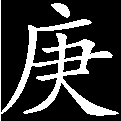
\includegraphics[width=3mm]{../Images/00004}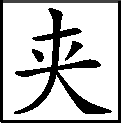
\includegraphics[width=3mm]{../Images/00012}\footnotesize \kaishu 作书者曾吃此亏,批书者亦曾吃此亏,故特于此注明,使后人深思默戒。脂砚斋。}薛姨妈听了,思忖半晌说道:``倒是你说的是。花两个钱,叫他学些乖来也值了。''商议已定,一宿无话。

至次日,薛姨妈命人请了张德辉来,在书房中命薛蟠款待酒饭,自己在后廊下,隔着窗子,向里千言万语嘱托张德辉照管薛蟠。张德辉满口应承,吃过饭告辞,又回说:``十四日是上好出行日期,大世兄即刻打点行李,雇下骡子,十四一早就长行了。''薛蟠喜之不尽,将此话告诉了薛姨妈。薛姨妈便和宝钗香菱并两个老年的嬷嬷连日打点行装,派下薛蟠之乳父老苍头一名,当年谙事旧仆二名,外有薛蟠随身常使小厮二人,主仆一共六人,雇了三辆大车,单拉行李使物,又雇了四个长行骡子。薛蟠自骑一匹家内养的铁青大走骡,外备一匹坐马。诸事完毕,薛姨妈宝钗等连夜劝戒之言,自不必备说。

至十三日,薛蟠先去辞了他舅舅,然后过来辞了贾宅诸人。贾珍等未免又有饯行之说,也不必细述。至十四日一早,薛姨妈宝钗等直同薛蟠出了仪门,母女两个四只泪眼看他去了,方回来。

薛姨妈上京带来的家人不过四五房,并两三个老嬷嬷小丫头,今跟了薛蟠一去,外面只剩了一两个男子。因此薛姨妈即日到书房,将一应陈设玩器并帘幔等物尽行搬了进来收贮,命那两个跟去的男子之妻一并也进来睡觉。又命香菱将他屋里也收拾严紧,``将门锁了,晚间和我去睡。''宝钗道:``妈既有这些人作伴,不如叫菱姐姐和我作伴去。我们园里又空,夜长了,我每夜作活,越多一个人岂不越好。''薛姨妈听了,笑道:``正是我忘了,原该叫他同你去才是。我前日还同你哥哥说,文杏又小,道三不着两,莺儿一个人不够伏侍的,还要买一个丫头来你使。''宝钗道:``买的不知底里,倘或走了眼,花了钱小事,没的淘气。倒是慢慢的打听着,有知道来历的,买个还罢了。''{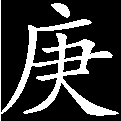
\includegraphics[width=3mm]{../Images/00004}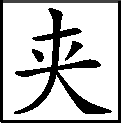
\includegraphics[width=3mm]{../Images/00012}\footnotesize \kaishu 闲言过耳无迹,然已伏下一事矣。}一面说,一面命香菱收拾了衾褥妆奁,命一个老嬷嬷并臻儿送至蘅芜苑去,然后宝钗和香菱才同回园中来。{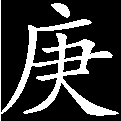
\includegraphics[width=3mm]{../Images/00004}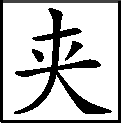
\includegraphics[width=3mm]{../Images/00012}\footnotesize \kaishu 细想香菱之为人也,根基不让迎、探,容貌不让凤、秦,端雅不让纨、钗,风流不让湘、黛,贤惠不让袭、平,所惜者青年罹祸,命运乖蹇,至为侧室,且虽曾读书,不能与林、湘辈并驰于海棠之社耳。然此一人岂可不入园哉?故欲令入园,终无可入之隙,筹划再四,欲令入园必呆兄远行后方可。然阿呆兄又如何方可远行?曰名不可,利不可,正事不可,必得万人想不到,自己忽一发机之事方可。因此思及``情''之一字乃呆素所误者,故借``情误''二字生出一事,使阿呆游艺之志已坚,则菱卿入园之隙方妥。回思因欲香菱入园,是写阿呆情误,因欲阿呆情误,先写一赖尚荣,实委婉严密之甚也。脂砚斋评。}

香菱道:``我原要和奶奶说的,大爷去了,我和姑娘作伴儿去。又恐怕奶奶多心,说我贪着园里来顽;谁知你竟说了。''宝钗笑道:``我知道你心里羡慕这园子不是一日两日了,只是没个空儿。就每日来一趟,慌慌张张的,也没趣儿。所以趁着机会,越性住上一年,我也多个作伴的,你也遂了心。''香菱笑道:``好姑娘,你趁着这个功夫,教给我作诗罢。''{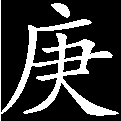
\includegraphics[width=3mm]{../Images/00004}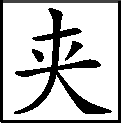
\includegraphics[width=3mm]{../Images/00012}\footnotesize \kaishu 写得何其有趣,今忽见菱卿此句,合卷从纸上另走出一姣小美人来,并不是湘、林、探、凤等一样口气声色。真神骏之技,虽驰驱万里而不见有倦怠之色。}宝钗笑道:``我说你`得陇望蜀'呢。我劝你今儿头一日进来,先出园东角门,从老太太起,各处各人你都瞧瞧,问候一声儿,也不必特意告诉他们说搬进园来。若有提起因由,你只带口说我带了你进来作伴儿就完了。回来进了园,再到各姑娘房里走走。''

香菱应着才要走时,只见平儿忙忙的走来。{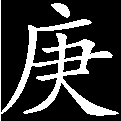
\includegraphics[width=3mm]{../Images/00004}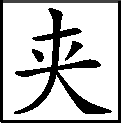
\includegraphics[width=3mm]{../Images/00012}\footnotesize \kaishu ``忙忙''二字奇,不知有何妙文。}香菱忙问了好,平儿只得陪笑相问。宝钗因向平儿笑道:``我今儿带了他来作伴儿,正要去回你奶奶一声儿。''平儿笑道:``姑娘说的是那里话?我竟没话答言了。''宝钗道:``这才是正理。店房也有个主人,庙里也有个住持。虽不是大事,到底告诉一声,便是园里坐更上夜的人知道添了他两个,也好关门候户的了。你回去告诉一声罢,我不打发人去了。''平儿答应着,因又向香菱笑道:``你既来了,也不拜一拜街坊邻舍去?''{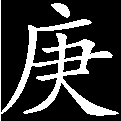
\includegraphics[width=3mm]{../Images/00004}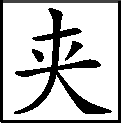
\includegraphics[width=3mm]{../Images/00012}\footnotesize \kaishu 是极,恰是戏言,实欲支出香菱去也。}宝钗笑道:``我正叫他去呢。''平儿道:``你且不必往我们家去,二爷病了在家里呢。''香菱答应着去了,先从贾母处来,不在话下。

且说平儿见香菱去了,便拉宝钗忙说道:``姑娘可听见我们的新闻了?''宝钗道:``我没听见新闻。因连日打发我哥哥出门,所以你们这里的事,一概也不知道,连姊妹们这两日也没见。''平儿笑道:``老爷把二爷打了个动不得,难道姑娘就没听见?''宝钗道:``早起恍惚听见了一句,也信不真。我也正要瞧你奶奶去呢,不想你来了。又是为了什么打他?''平儿咬牙骂道:``都是那贾雨村什么风村,半路途中那里来的饿不死的野杂种!认了不到十年,生了多少事出来!今年春天,老爷不知在那个地方看见了几把旧扇子,回家看家里所有收着的这些好扇子都不中用了,立刻叫人各处搜求。谁知就有一个不知死的冤家,混号儿世人叫他作石呆子,穷的连饭也没的吃,偏他家就有二十把旧扇子,死也不肯拿出大门来。二爷好容易烦了多少情,见了这个人,说之再三,把二爷请到他家里坐着,拿出这扇子略瞧了一瞧。据二爷说,原是不能再有的,全是湘妃、棕竹、麋鹿、玉竹的,皆是古人写画真迹,因来告诉了老爷。老爷便叫买他的,要多少银子给他多少。偏那石呆子说:`我饿死冻死,一千两银子一把我也不卖!'老爷没法子,天天骂二爷没能为。已经许了他五百两,先兑银子后拿扇子。他只是不卖,只说:`要扇子,先要我的命!'姑娘想想,这有什么法子?谁知雨村那没天理的听见了,便设了个法子,讹他拖欠了官银,拿他到衙门里去,说所欠官银,变卖家产赔补,把这扇子抄了来,作了官价送了来。那石呆子如今不知是死是活。老爷拿着扇子问着二爷说:`人家怎么弄了来?'二爷只说了一句:`为这点子小事,弄得人坑家败业,也不算什么能为!'老爷听了就生了气,说二爷拿话堵老爷,因此这是第一件大的。这几日还有几件小的,我也记不清,所以都凑在一处,就打起来了。也没拉倒用板子棍子,就站着,不知拿什么混打一顿,脸上打破了两处。我们听见姨太太这里有一种丸药,上棒疮的,姑娘快寻一丸子给我。''宝钗听了,忙命莺儿去要了一丸来与平儿。宝钗道:``既这样,替我问候罢,我就不去了。''平儿答应着去了,不在话下。

且说香菱见过众人之后,吃过晚饭,宝钗等都往贾母处去了,自己便往潇湘馆中来。此时黛玉已好了大半,见香菱也进园来住,自是欢喜。香菱因笑道:``我这一进来了,也得了空儿,好歹教给我作诗,就是我的造化了!''黛玉笑道:``既要作诗,你就拜我作师。我虽不通,大略也还教得起你。''香菱笑道:``果然这样,我就拜你作师。你可不许腻烦的。''黛玉道:``什么难事,也值得去学!不过是起承转合,当中承转是两副对子,平声对仄声,虚的对实的,实的对虚的,若是果有了奇句,连平仄虚实不对都使得的。''香菱笑道:``怪道我常弄一本旧诗偷空儿看一两首,又有对的极工的,又有不对的,又听见说`一三五不论,二四六分明'。看古人的诗上亦有顺的,亦有二四六上错了的,所以天天疑惑。如今听你一说,原来这些格调规矩竟是末事,只要词句新奇为上。''黛玉道:``正是这个道理。词句究竟还是末事,第一立意要紧。若意趣真了,连词句不用修饰,自是好的,这叫做`不以词害意'。''

香菱笑道:``我只爱陆放翁的诗`重帘不卷留香久,古砚微凹聚墨多',说的真有趣!''黛玉道:``断不可学这样的诗。你们因不知诗,所以见了这浅近的就爱,一入了这个格局,再学不出来的。你只听我说,你若真心要学,我这里有《王摩诘全集》,你且把他的五言律读一百首,细心揣摩透熟了,然后再读一二百首老杜的七言律,次再李青莲的七言绝句读一二百首。肚子里先有了这三个人作了底子,然后再把陶渊明、应玚、谢、阮、庾、鲍等人的一看。你又是一个极聪敏伶俐的人,不用一年的工夫,不愁不是诗翁了!''香菱听了,笑道:``既这样,好姑娘,你就把这书给我拿出来,我带回去夜里念几首也是好的。''黛玉听说,便命紫鹃将王右丞的五言律拿来,递与香菱,又道:``你只看有红圈的都是我选的,有一首念一首。不明白的问你姑娘,或者遇见我,我讲与你就是了。''香菱拿了诗,回至蘅芜苑中,诸事不顾,只向灯下一首一首的读起来。宝钗连催他数次睡觉,他也不睡。宝钗见他这般苦心,只得随他去了。

一日,黛玉方梳洗完了,只见香菱笑吟吟的送了书来,又要换杜律。黛玉笑道:``共记得多少首?''香菱笑道:``凡红圈选的我尽读了。''黛玉道:``可领略了些滋味没有?''香菱笑道:``领略了些滋味,不知可是不是,说与你听听。''黛玉笑道:``正要讲究讨论,方能长进。你且说来我听。''香菱笑道:``据我看来,诗的好处,有口里说不出来的意思,想去却是逼真的。有似乎无理的,想去竟是有理有情的。''黛玉笑道:``这话有了些意思,但不知你从何处见得?''香菱笑道:``我看他《塞上》一首,那一联云:`大漠孤烟直,长河落日圆。'想来烟如何直?日自然是圆的:这`直'字似无理,`圆'字似太俗。合上书一想,倒像是见了这景的。若说再找两个字换这两个,竟再找不出两个字来。再还有`日落江湖白,潮来天地青',这`白'`青'两个字也似无理。想来,必得这两个字才形容得尽,念在嘴里倒像有几千斤重的一个橄榄。还有`渡头馀落日,墟里上孤烟',这`馀'字和`上'字,难为他怎么想来!我们那年上京来,那日下晚便湾住船,岸上又没有人,只有几棵树,远远的几家人家作晚饭,那个烟竟是碧青,连云直上。谁知我昨日晚上读了这两句,倒像我又到了那个地方去了。''

正说着,宝玉和探春也来了,也都入坐听他讲诗。宝玉笑道:``既是这样,也不用看诗。会心处不在多,听你说了这两句,可知三昧你已得了。''黛玉笑道:``你说他这`上孤烟'好,你还不知他这一句还是套了前人的来。我给你这一句瞧瞧,更比这个淡而现成。''说着便把陶渊明的``暧暧远人村,依依墟里烟''翻了出来,递与香菱。香菱瞧了,点头叹赏,笑道:``原来`上'字是从`依依'两个字上化出来的。''宝玉大笑道:``你已得了,不用再讲,越发倒学杂了。你就作起来,必是好的。''探春笑道:``明儿我补一个柬来,请你入社。''香菱笑道:``姑娘何苦打趣我,我不过是心里羡慕,才学着顽罢了。''探春黛玉都笑道:``谁不是顽?难道我们是认真作诗呢!若说我们认真成了诗,出了这园子,把人的牙还笑倒了呢。''宝玉道:``这也算自暴自弃了。前日我在外头和相公们商议画儿,他们听见咱们起诗社,求我把稿子给他们瞧瞧。我就写了几首给他们看看,谁不真心叹服。他们都抄了刻去了。''探春黛玉忙问道:``这是真话么?''宝玉笑道:``说谎的是那架上的鹦哥。''黛玉探春听说,都道:``你真真胡闹!且别说那不成诗,便是成诗,我们的笔墨也不该传到外头去。''宝玉道:``这怕什么!古来闺阁中的笔墨不要传出去,如今也没有人知道了。''说着,只见惜春打发了入画来请宝玉,宝玉方去了。香菱又逼着黛玉换出杜律来,又央黛玉探春二人:``出个题目,让我诌去,诌了来,替我改正。''黛玉道:``昨夜的月最好,我正要诌一首,竟未诌成,你竟作一首来。`十四寒'的韵,由你爱用那几个字去。''

香菱听了,喜的拿回诗来,又苦思一回作两句诗,又舍不得杜诗,又读两首。如此茶饭无心,坐卧不定。宝钗道:``何苦自寻烦恼。都是颦儿引的你,我和他算账去。你本来呆头呆脑的,再添上这个,越发弄成个呆子了。''{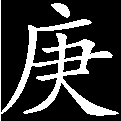
\includegraphics[width=3mm]{../Images/00004}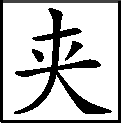
\includegraphics[width=3mm]{../Images/00012}\footnotesize \kaishu ``呆头呆脑的'',有趣之至!最恨野史,有一百个女子,皆曰``聪敏伶俐'',究竟看来,他行为也只平平。今以``呆''字为香菱定评,何等妩媚之至也。}香菱笑道:``好姑娘,别混我。''{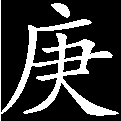
\includegraphics[width=3mm]{../Images/00004}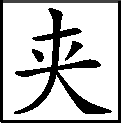
\includegraphics[width=3mm]{../Images/00012}\footnotesize \kaishu 如闻如见。}一面说,一面作了一首,先与宝钗看。宝钗看了笑道:``这个不好,不是这个作法。你别怕臊,只管拿了给他瞧去,看他是怎么说。''香菱听了,便拿了诗找黛玉。黛玉看时,只见写道是:

月挂中天夜色寒,清光皎皎影团团。

诗人助兴常思玩,野客添愁不忍观。

翡翠楼边悬玉镜,珍珠帘外挂冰盘。

良宵何用烧银烛,晴彩辉煌映画栏。

黛玉笑道:``意思却有,只是措词不雅。皆因你看的诗少,被他缚住了。把这首丢开,再作一首。只管放开胆子去作。''

香菱听了,默默的回来,越性连房也不入,只在池边树下,或坐在山石上出神,或蹲在地下抠土,来往的人都诧异。李纨、宝钗、探春、宝玉等听得此信,都远远的站在山坡上瞧着他。只见他皱一回眉,又自己含笑一回。宝钗笑道:``这个人定要疯了!昨夜嘟嘟哝哝直闹到五更天才睡下,没一顿饭的工夫天就亮了。我就听见他起来了,忙忙碌碌梳了头就找颦儿去。一回来了,呆了一日,作了一首又不好,这会子自然另作呢。''宝玉笑道:``这正是`地灵人杰',老天生人再不虚赋情性的。我们成日叹说可惜他这么个人竟俗了,谁知到底有今日。可见天地至公。''宝钗笑道:``你能够像他这苦心就好了,学什么有个不成的。''宝玉不答。

只见香菱兴兴头头的又往黛玉那边去了。探春笑道:``咱们跟了去,看他有些意思没有。''说着,一齐都往潇湘馆来。只见黛玉正拿着诗和他讲究。众人因问黛玉作的如何。黛玉道:``自然算难为他了,只是还不好。这一首过于穿凿了,还得另作。''众人因要诗看时,只见作道:

非银非水映窗寒,试看晴空护玉盘。

淡淡梅花香欲染,丝丝柳带露初干。

只疑残粉涂金砌,恍若轻霜抹玉栏。

梦醒西楼人迹绝,馀容犹可隔帘看。

宝钗笑道:``不像吟月了,月字底下添一个`色'字倒还使得,你看句句倒是月色。这也罢了,原来诗从胡说来,再迟几天就好了。''香菱自为这首妙绝,听如此说,自己扫了兴,不肯丢开手,便要思索起来。因见他姊妹们说笑,便自己走至阶前竹下闲步,挖心搜胆,耳不旁听,目不别视。一时探春隔窗笑说道:``菱姑娘,你闲闲罢。''香菱怔怔答道:```闲'字是`十五删'的,你错了韵了。''众人听了,不觉大笑起来。宝钗道:``可真是诗魔了。都是颦儿引的他!''黛玉笑道:``圣人说:`诲人不倦。'他又来问我,我岂有不说之理。''李纨笑道:``咱们拉了他往四姑娘房里去,引他瞧瞧画儿,叫他醒一醒才好。''

说着,真个出来拉了他过藕香榭,至暖香坞中。惜春正乏倦,在床上歪着睡午觉,画缯立在壁间,用纱罩着。众人唤醒了惜春,揭纱看时,十停方有了三停。香菱见画上有几个美人,因指着笑道:``这一个是我们姑娘,那一个是林姑娘。''探春笑道:``凡会作诗的都画在上头,快学罢。''说着,顽笑了一回。

各自散后,香菱满心中还是想诗。至晚间对灯出了一回神,至三更以后上床卧下,两眼鳏鳏,直到五更方才朦胧睡去了。一时天亮,宝钗醒了,听了一听,他安稳睡了,心下想:``他翻腾了一夜,不知可作成了?这会子乏了,且别叫他。''正想着,只听香菱从梦中笑道:``可是有了,难道这一首还不好?''宝钗听了,又是可叹,又是可笑,连忙唤醒了他,问他:``得了什么?你这诚心都通了仙了。学不成诗,还弄出病来呢。''一面说,一面梳洗了,会同姊妹往贾母处来。原来香菱苦志学诗,精血诚聚,日间做不出,忽于梦中得了八句。梳洗已毕,便忙录出来,自己并不知好歹,便拿来又找黛玉。刚到沁芳亭,只见李纨与众姊妹方从王夫人处回来,宝钗正告诉他们说他梦中作诗说梦话。{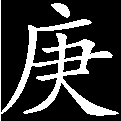
\includegraphics[width=3mm]{../Images/00004}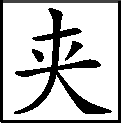
\includegraphics[width=3mm]{../Images/00012}\footnotesize \kaishu 一部大书,起是梦,宝玉情是梦,贾瑞淫又是梦,秦之家计长策又是梦,今作诗也是梦,一并``风月鉴''亦从梦中所有,故``红楼梦''也。余今批评亦在梦中,特为梦中之人特作此一大梦也。脂砚斋。}众人正笑,抬头见他来了,便都争着要诗看。且听下回分解。

{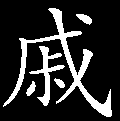
\includegraphics[width=3mm]{../Images/00005}总评:一扇之微,而害人如此其毒。藏之者故是无味,构求者更觉可笑。多少没天理处,全不自觉。可见好爱之端,断不可生。求古董于古坟,争盆景而荡产,势所必至,可不慎诸。}
